\subsection{Langkah Praktikum: Selection Sort}

\subsubsection*{Flowchart}
\begin{figure}[H]
    \centering
    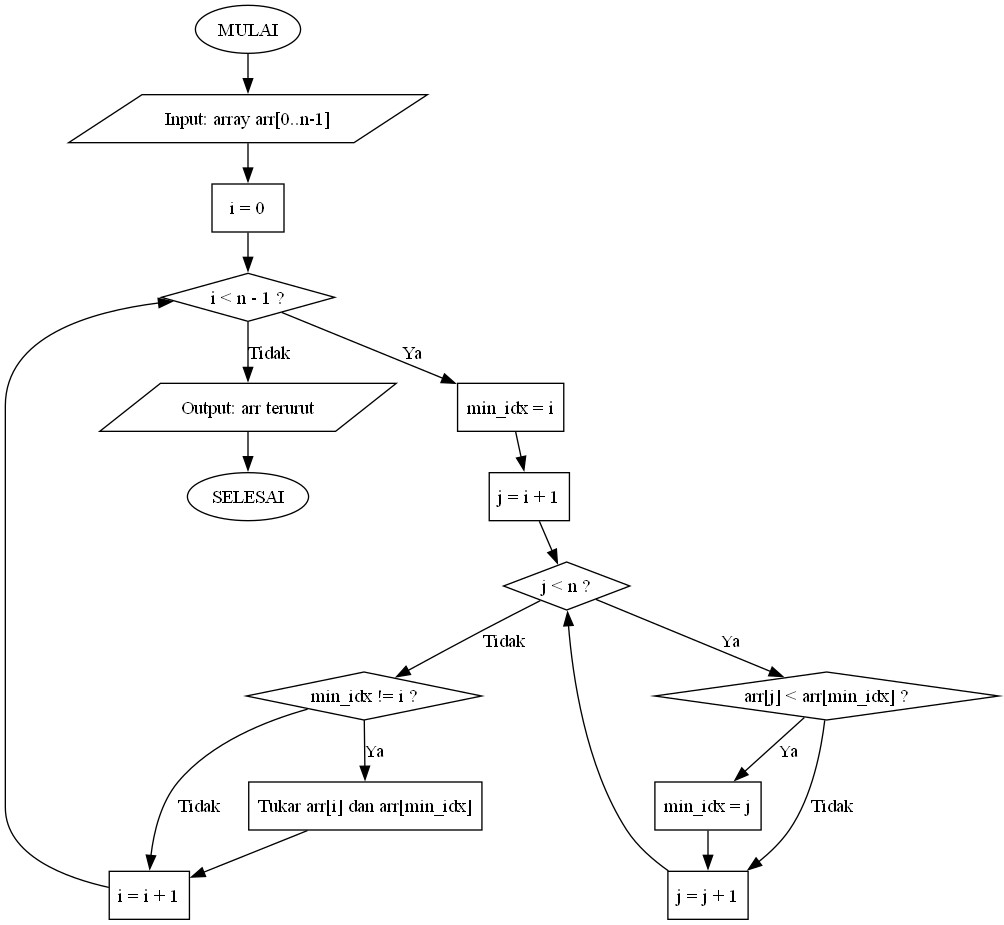
\includegraphics[width=0.65\textwidth]{figures/praktikum1/flowchart_selection_sort.png}
    \caption{Flowchart Algoritma Selection Sort}
\end{figure}

\subsubsection*{Source Code Python}
\begin{lstlisting}[basicstyle=\ttfamily\scriptsize, frame=single, backgroundcolor=\color{white}, numbers=none, keywordstyle=\color{black}, commentstyle=\color{black}, stringstyle=\color{black}, breaklines=true]
def selection_sort(arr):
    """
    Mengurutkan array dengan algoritma Selection Sort.
    Setiap pass mencari elemen terkecil dari sisa array
    lalu menukarnya ke posisi yang tepat.
    """
    n = len(arr)
    total_comparisons = 0
    total_swaps = 0
    print(f"Array awal : {arr}")
    print("-" * 55)

    for i in range(n - 1):
        # Asumsikan elemen terkecil ada di posisi i
        min_idx = i
        pass_comparisons = 0
        pass_swaps = 0

        # Cari elemen terkecil dari i+1 hingga akhir array
        for j in range(i + 1, n):
            pass_comparisons += 1
            if arr[j] < arr[min_idx]:
                min_idx = j

        # Tukar elemen terkecil ke posisi i (jika berbeda)
        if min_idx != i:
            arr[i], arr[min_idx] = arr[min_idx], arr[i]
            pass_swaps += 1

        total_comparisons += pass_comparisons
        total_swaps += pass_swaps

        print(f"Pass {i + 1:2d} | Array: {arr} | "
              f"Perbandingan: {pass_comparisons:2d} | "
              f"Pertukaran: {pass_swaps}")
        print("-" * 55)

    print(f"Array akhir : {arr}")
    print(f"Total perbandingan : {total_comparisons}")
    print(f"Total pertukaran   : {total_swaps}")
    return arr
\end{lstlisting}

\subsubsection*{Analisis}
\textbf{Jawaban 1: Jumlah operasi perbandingan untuk setiap pass ke-i}\\
Pada pass ke-i (i dari 0 sampai n-2), algoritma mencari elemen minimum dari posisi i+1 hingga n-1. Jumlah perbandingan pada setiap pass disajikan pada Tabel \ref{tab:perbandingan_selection}:

\begin{table}[H]
    \centering
    \caption{Operasi Perbandingan Per Pass Selection Sort}
    \label{tab:perbandingan_selection}
    \begin{tabular}{ccc}
    \toprule
    \textbf{Pass ke-i} & \textbf{Rentang Pencarian} & \textbf{Perbandingan} \\ \midrule
    0 & A[1] hingga A[4] & 4 \\
    1 & A[2] hingga A[4] & 3 \\
    2 & A[3] hingga A[4] & 2 \\
    3 & A[4] hingga A[4] & 1 \\ \bottomrule
    \end{tabular}
\end{table}

\textbf{Jawaban 2: Jumlah operasi pertukaran elemen}\\
Setiap pass melakukan paling banyak 1 kali pertukaran, hanya apabila elemen minimum (min\_idx) bukan berada di posisi i. Pertukaran minimum 0 kali (array sudah terurut) dan maksimum n-1 kali. Pada Kasus Uji 1 dengan n=5, total pertukaran = 3 dari 4 pass.

\textbf{Jawaban 3: Derivasi kompleksitas waktu}\\
Total perbandingan dijumlahkan dari seluruh pass:
\[ T(n) = (n-1) + (n-2) + ... + 1 = n(n-1) / 2 \]
Untuk n=5: T(5) = 5 $\times$ 4 / 2 = 10, sesuai output program. Suku dominan adalah $n^2$, sehingga kompleksitas waktu Selection Sort adalah $O(n^2)$.


\subsection{Post Test: Insertion Sort}

\subsubsection*{Flowchart}
\begin{figure}[H]
    \centering
    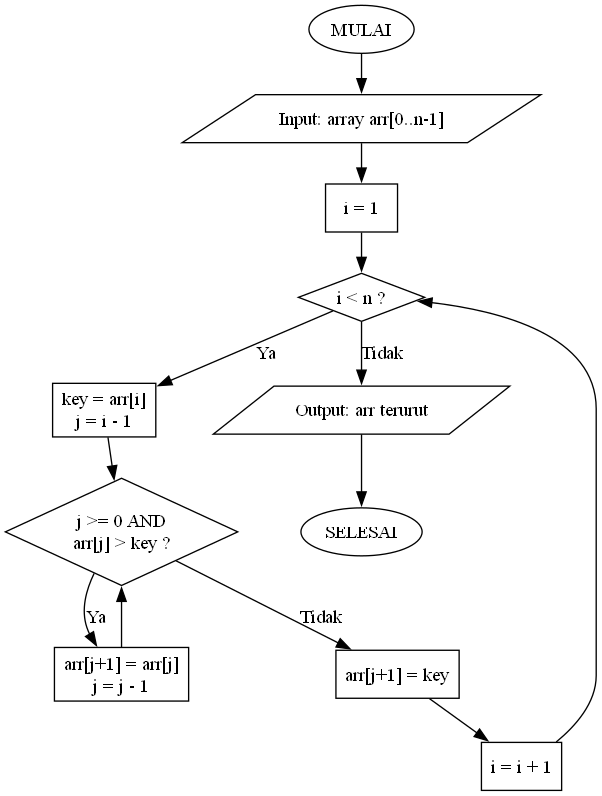
\includegraphics[width=0.65\textwidth]{figures/praktikum1/flowchart_insertion_sort.png}
    \caption{Flowchart Algoritma Insertion Sort}
\end{figure}

\subsubsection*{Source Code Python}
\begin{lstlisting}[basicstyle=\ttfamily\scriptsize, frame=single, backgroundcolor=\color{white}, numbers=none, keywordstyle=\color{black}, commentstyle=\color{black}, stringstyle=\color{black}, breaklines=true]
def insertion_sort(arr):
    """
    Mengurutkan array dengan algoritma Insertion Sort.
    Setiap elemen disisipkan ke posisi yang tepat
    di dalam bagian array yang sudah terurut.
    """
    n = len(arr)
    total_comparisons = 0
    total_shifts = 0
    print(f"Array awal : {arr}")
    print("-" * 60)

    for i in range(1, n):
        key = arr[i]
        j = i - 1
        pass_comparisons = 0
        pass_shifts = 0

        # Geser elemen yang lebih besar dari key ke kanan
        while j >= 0 and arr[j] > key:
            arr[j + 1] = arr[j]
            j -= 1
            pass_comparisons += 1
            pass_shifts += 1

        # Hitung perbandingan terakhir (kondisi berhenti)
        if j >= 0:
            pass_comparisons += 1

        # Sisipkan key ke posisi yang tepat
        arr[j + 1] = key
        total_comparisons += pass_comparisons
        total_shifts += pass_shifts

        print(f"Pass {i:2d} | key={key:3d} | Array: {arr} | "
              f"Perbandingan: {pass_comparisons} | "
              f"Pergeseran: {pass_shifts}")
        print("-" * 60)

    print(f"Array akhir        : {arr}")
    print(f"Total perbandingan : {total_comparisons}")
    print(f"Total pergeseran   : {total_shifts}")
    return arr
\end{lstlisting}

\subsubsection*{Analisis}
\textbf{Jawaban 1: Kompleksitas waktu Insertion Sort}
\begin{itemize}
    \item \textbf{Best Case O(n):} Array sudah terurut. Setiap elemen hanya dibandingkan sekali, tidak ada pergeseran. T(n) = n-1.
    \item \textbf{Worst Case O(n$^2$):} Array terurut terbalik. Elemen ke-i harus digeser i kali. T(n) = 1+2+...+(n-1) = n(n-1)/2.
    \item \textbf{Average Case O(n$^2$):} Rata-rata elemen ke-i melakukan i/2 perbandingan. T(n) $\approx$ n(n-1)/4.
\end{itemize}

\textbf{Jawaban 2: Perbandingan Selection Sort vs Insertion Sort}
Tabel \ref{tab:komparasi_sort} merangkum perbedaan karakteristik antara kedua algoritma pengurutan tersebut:

\begin{table}[H]
    \centering
    \caption{Perbandingan Selection Sort dan Insertion Sort}
    \label{tab:komparasi_sort}
    \begin{tabular}{lll}
    \toprule
    \textbf{Aspek} & \textbf{Insertion Sort} & \textbf{Selection Sort} \\ \midrule
    Best Case & O(n) --- adaptif & O(n$^2$) --- tidak adaptif \\
    Worst Case & O(n$^2$) & O(n$^2$) \\
    Average Case & O(n$^2$) & O(n$^2$) \\
    Pertukaran/Geser & Banyak (pergeseran) & Sedikit (maks. n-1) \\
    Stabilitas & Stabil & Tidak Stabil \\
    Adaptivitas & Adaptif & Tidak Adaptif \\ \bottomrule
    \end{tabular}
\end{table}

\textbf{Kesimpulan:} Insertion Sort lebih mangkus pada data yang hampir terurut karena bersifat adaptif dengan best case O(n). Selection Sort lebih unggul dalam minimasi pertukaran (maks. n-1 swap), cocok ketika operasi swap memiliki biaya mahal. Pada data acak berukuran besar keduanya setara di $O(n^2)$.
